\chapter{Dialect Formation Across Populations (RQ2)}
\label{ch:rq2}

\providecommand{\missingfigure}[1]{%
\fcolorbox{red}{white}{%
\parbox[c][0.14\textheight][c]{0.9\textwidth}{\centering\textcolor{red}{Placeholder figure\\\texttt{\detokenize{#1}}}}%
}%
}

This chapter tests the second research question: whether populations of PACE agents trained on the same Zipfian concentration $\alpha$ but on different rankings develop systematically different abstraction libraries. We keep the concentration profile fixed and vary only the random permutation that determines which shape pairs sit at the top of the ranking. This lets us ask whether two populations exposed to the same level of frequency concentration but to different top pairs converge on the same abstractions or develop systematically different ones.

Section~\ref{sec:rq2-motivation} motivates the dialect formation framing, situating it against the human convention literature reviewed in Chapter~\ref{ch:background}, especially work on how repeated interaction stabilises pair-specific referential conventions~\cite{hawkins_convention-formation_2017,hawkins_characterizing_2020}. Section~\ref{sec:rq2-methodology} introduces the metrics we use to compare abstraction libraries and the null model we use to separate genuine convergence from chance agreement. Section~\ref{sec:rq2-results} reports the main quantitative result: mean pairwise overlap as a function of $\alpha$, together with the null model comparison and the dialect signal. Section~\ref{sec:rq2-heatmaps} looks at how the aggregate picture is distributed across individual seed pairs, through pairwise overlap heatmaps at four representative $\alpha$ values. Section~\ref{sec:rq2-qualitative} examines the abstractions themselves, qualitatively, at a moderate $\alpha$, and shows how they track the structural properties of the seed-specific top pairs. Section~\ref{sec:rq2-intraseed} briefly compares the cross-seed picture to how a single seed's library changes when $\alpha$ itself varies. Section~\ref{sec:rq2-summary} discusses the findings and connects them to Chapter~\ref{ch:rq3}.

\section{Motivation}
\label{sec:rq2-motivation}

The dialect question grows naturally out of what Chapter~\ref{ch:experimental} established. RQ1 showed that the concentration parameter $\alpha$ shapes how many abstractions the bandit adopts, how compressed the emergent language becomes, and how unevenly the vocabulary is used. RQ2 asks a complementary but distinct question: with $\alpha$ held constant, does the identity of the top-ranked pairs determine which specific abstractions emerge? If the answer is yes, then the vocabulary a population develops is specific to that population, not a universal response to the pressure that shaped it.

The question matters both theoretically and methodologically. Theoretically, the dialect hypothesis gives a finer-grained alternative to treating properties such as compositionality or irregularity as global features of an emergent language: populations can share the same distributional profile and still develop different libraries when their top pairs differ. Methodologically, cross-population communication only becomes interpretable once we know whether the vocabularies really diverge, and at which concentration levels. The analysis in this chapter therefore provides the library-level background needed for Chapter~\ref{ch:rq3}, where communication difficulty turns out to depend on more than raw library divergence.

The seed-based ranking mechanism introduced in Chapter~\ref{ch:technical} gives us direct experimental control over this question. For a given $\alpha$, all 20 seeds see a Zipfian distribution with the same shape---this follows directly from the way we generate the datasets. By ranking we mean the specific assignment of shape pairs to positions in that distribution: different rankings put different pairs at the top. This decoupling of concentration from identity is what makes the dialect analysis possible in the first place.

\section{Methodology}
\label{sec:rq2-methodology}

\subsection{Measuring Overlap Between Libraries}
\label{sec:rq2-overlap}

For every combination of $\alpha$ and seed, we extract the set of abstractions the bandit adopted during training. Each abstraction is represented as a sequence of primitive actions, normalised to remove whitespace, so that two seeds adopting the same primitive sequence produce the same string regardless of the token index that each seed's DSL happens to have assigned to it. The adopted library for a run is therefore a set of primitive-sequence strings, and two runs can be compared by computing standard set-theoretic overlap measures on these sets.

We use two complementary metrics. The Jaccard index is the size of the intersection divided by the size of the union, and it ranges from zero, for no shared abstractions, to one, for identical libraries. Jaccard penalises differences both in content and in size: two libraries can score low either because they disagree on which abstractions to include or because one is much larger than the other. The same index has been used similarly to quantify lexical alignment between interacting human partners~\cite{ji_ad_2025}, although here the objects being compared are abstraction libraries rather than sets of natural-language words.

The overlap coefficient is the size of the intersection divided by the size of the smaller library. It also ranges from zero to one, but it does not penalise size differences. If one library is a subset of another, the overlap coefficient is one regardless of the size gap. This metric is useful for detecting cases where two seeds agree on a core set of abstractions but one of them additionally adopts extras that the other does not.

For both metrics, we treat any comparison involving an empty library as a missing value rather than as zero or one. Two seeds that adopted nothing have not ``agreed perfectly'': they have failed to learn, which is a different phenomenon and should not contaminate the overlap signal. In practice this rule only affects a small number of comparisons at the very top of the $\alpha$ range.

For each $\alpha$, we compute pairwise overlap for all 190 unordered pairs of seeds, and average across pairs to obtain the mean overlap at that $\alpha$. The standard deviation across pairs gives us a measure of variability.

\subsection{Null Model}
\label{sec:rq2-null}

A positive mean overlap on its own does not demonstrate that populations converge on shared conventions, because two libraries may overlap simply because the candidate pool is small. The null model estimates how much overlap two random populations would show if they drew abstractions independently from the same pool. Specifically, we pool all abstractions adopted across the 20 seeds at a given $\alpha$. For each pair of seeds, we then sample two random subsets without replacement, matching the actual library sizes of the two seeds, and compute their Jaccard index and overlap coefficient. Averaging over 1000 repetitions per pair and then across all 190 seed pairs gives the null overlap at that $\alpha$.

The signed difference between observed and null overlap is the quantity of primary interest, and we call it the dialect signal. When the dialect signal is positive, seeds share more abstractions than chance would predict, meaning that some abstractions are universally attractive across populations. When the dialect signal is negative, seeds share fewer abstractions than chance would predict, meaning that each population is locking in on its own idiosyncratic candidates. A signal close to zero means that the observed overlap is indistinguishable from random sampling.

\subsection{A Note on Reliability at High $\alpha$}
\label{sec:rq2-reliability}

At high $\alpha$ the candidate pool shrinks and the libraries individual seeds adopt become small. Computing overlap on small sets is intrinsically noisy: a single shared or non-shared abstraction can shift the Jaccard index by a large amount. To check whether the high-$\alpha$ results are still informative, we track at each $\alpha$ how many of the 20 seeds adopted at least three abstractions. This threshold holds throughout the range: at every $\alpha$ value, between 16 and 20 of the 20 seeds meet the threshold, with the lowest count of 17 occurring at $\alpha = 0.30$ and $\alpha = 0.45$. The statistical reliability of the overlap estimates is therefore comparable across the full experimental range, and we report results for all $\alpha$ values without further filtering.

The interpretive value at high $\alpha$ is a different question, and we return to it in Section~\ref{sec:rq2-summary}. The library at high $\alpha$ is not less reliable than at low $\alpha$, but it is smaller and more tightly tied to a handful of pairs, and that changes what the overlap numbers mean.

\section{Pairwise Overlap Across $\alpha$}
\label{sec:rq2-results}

Figure~\ref{fig:rq2-overlap-vs-alpha} shows the mean pairwise overlap as a function of $\alpha$, computed separately for the Jaccard index and the overlap coefficient, with shaded bands indicating one standard deviation across the 190 seed pairs. The null model is overlaid as a dashed line in both panels.

\begin{figure}[t]
    \centering
    \IfFileExists{images/overlap_vs_alpha.png}{%
        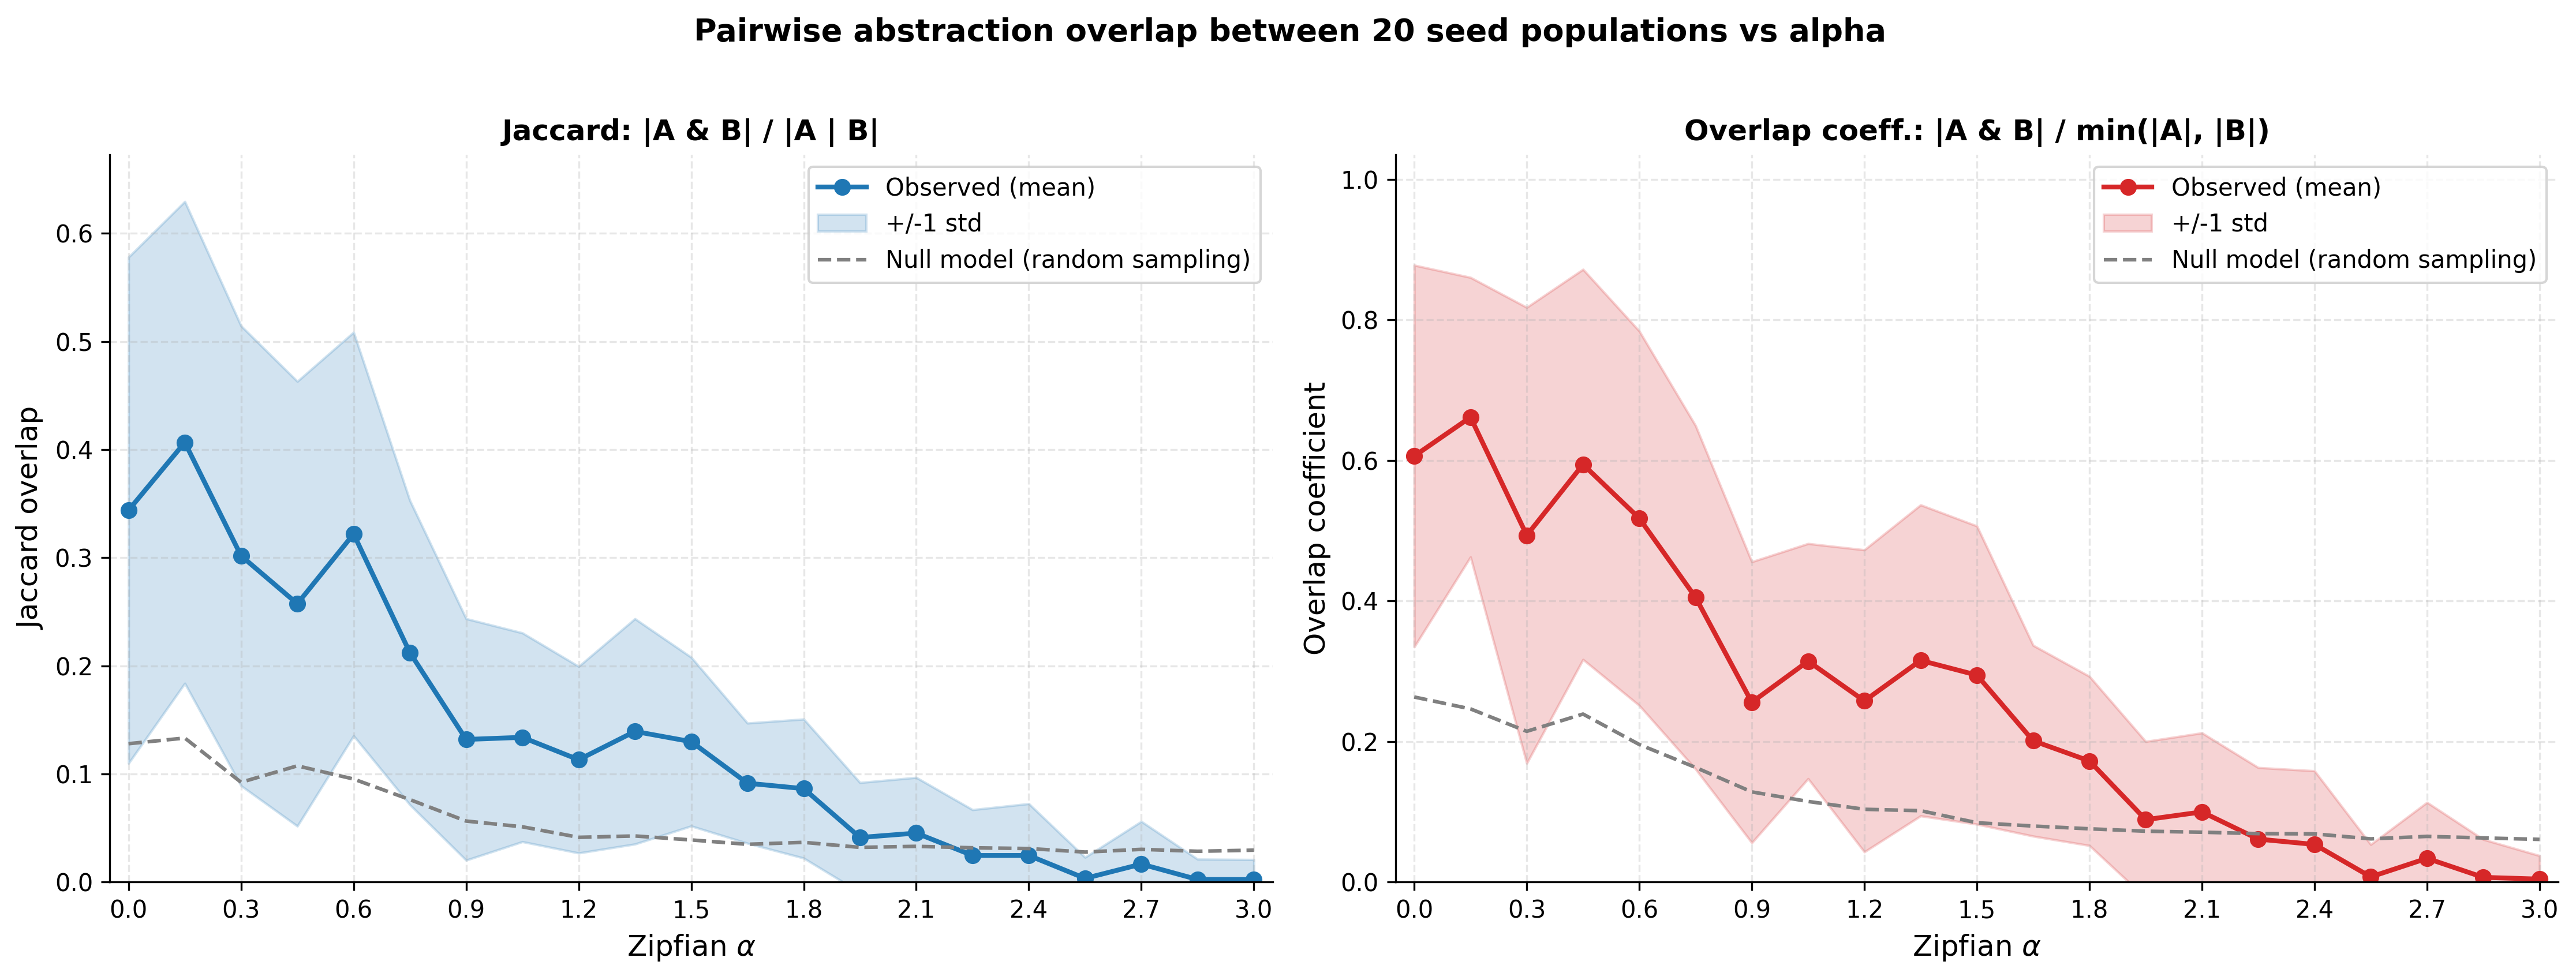
\includegraphics[width=0.95\textwidth]{images/overlap_vs_alpha.png}%
    }{%
        \missingfigure{images/overlap_vs_alpha.png}%
    }
    \caption{Mean pairwise overlap between abstraction libraries as a function of $\alpha$, reported for the Jaccard index and the overlap coefficient. Dashed lines indicate the corresponding null-model expectation.}
    \label{fig:rq2-overlap-vs-alpha}
\end{figure}

The two metrics tell consistent stories with different magnitudes. The Jaccard overlap starts at approximately 0.34 at $\alpha = 0.00$ and decreases monotonically with $\alpha$, reaching 0.13 at $\alpha = 0.90$, 0.05 at $\alpha = 2.10$, and approximately zero at $\alpha = 3.00$. The overlap coefficient is uniformly higher, as expected since it does not penalise size differences. It starts at approximately 0.61 at $\alpha = 0.00$, falls more gradually through the moderate range, and converges to near zero at $\alpha = 3.00$. Both metrics follow the same trajectory: high overlap at low concentration, gradual decrease through the moderate range, and collapse at high concentration.

The Spearman rank correlation between $\alpha$ and mean Jaccard overlap is $-0.979$ with $p < 10^{-6}$, and the correlation with the overlap coefficient is $-0.973$ with $p < 10^{-6}$. Unlike RQ1, where the pattern was non-monotone and no single correlation could summarise it, here the relationship is genuinely monotone and the Spearman correlation captures it faithfully.

The null model overlay reveals an additional layer of structure. At low and moderate $\alpha$, the observed Jaccard overlap sits well above the null. The gap between observed and null is largest at low $\alpha$: the observed Jaccard exceeds the null by approximately 0.22 at $\alpha = 0.00$ and by 0.23 at $\alpha = 0.60$. The gap narrows through the moderate range but stays positive up to $\alpha = 2.10$. At $\alpha = 2.25$ the observed and null curves cross, and for $\alpha \geq 2.40$ the observed overlap sits slightly below the null.

Figure~\ref{fig:rq2-dialect-signal} shows the dialect signal directly, as the difference between observed and null. The Jaccard dialect signal is positive throughout the low and moderate range, peaks around $\alpha = 0.60$, and decreases monotonically toward zero at around $\alpha \approx 2.19$. Beyond this crossover the signal becomes slightly negative, meaning that seeds at very high $\alpha$ share fewer abstractions than chance sampling would predict. The overlap coefficient signal shows the same crossover at a similar $\alpha$, with a slightly more pronounced negative excursion.

\begin{figure}[t]
    \centering
    \IfFileExists{images/overlap_minus_null.png}{%
        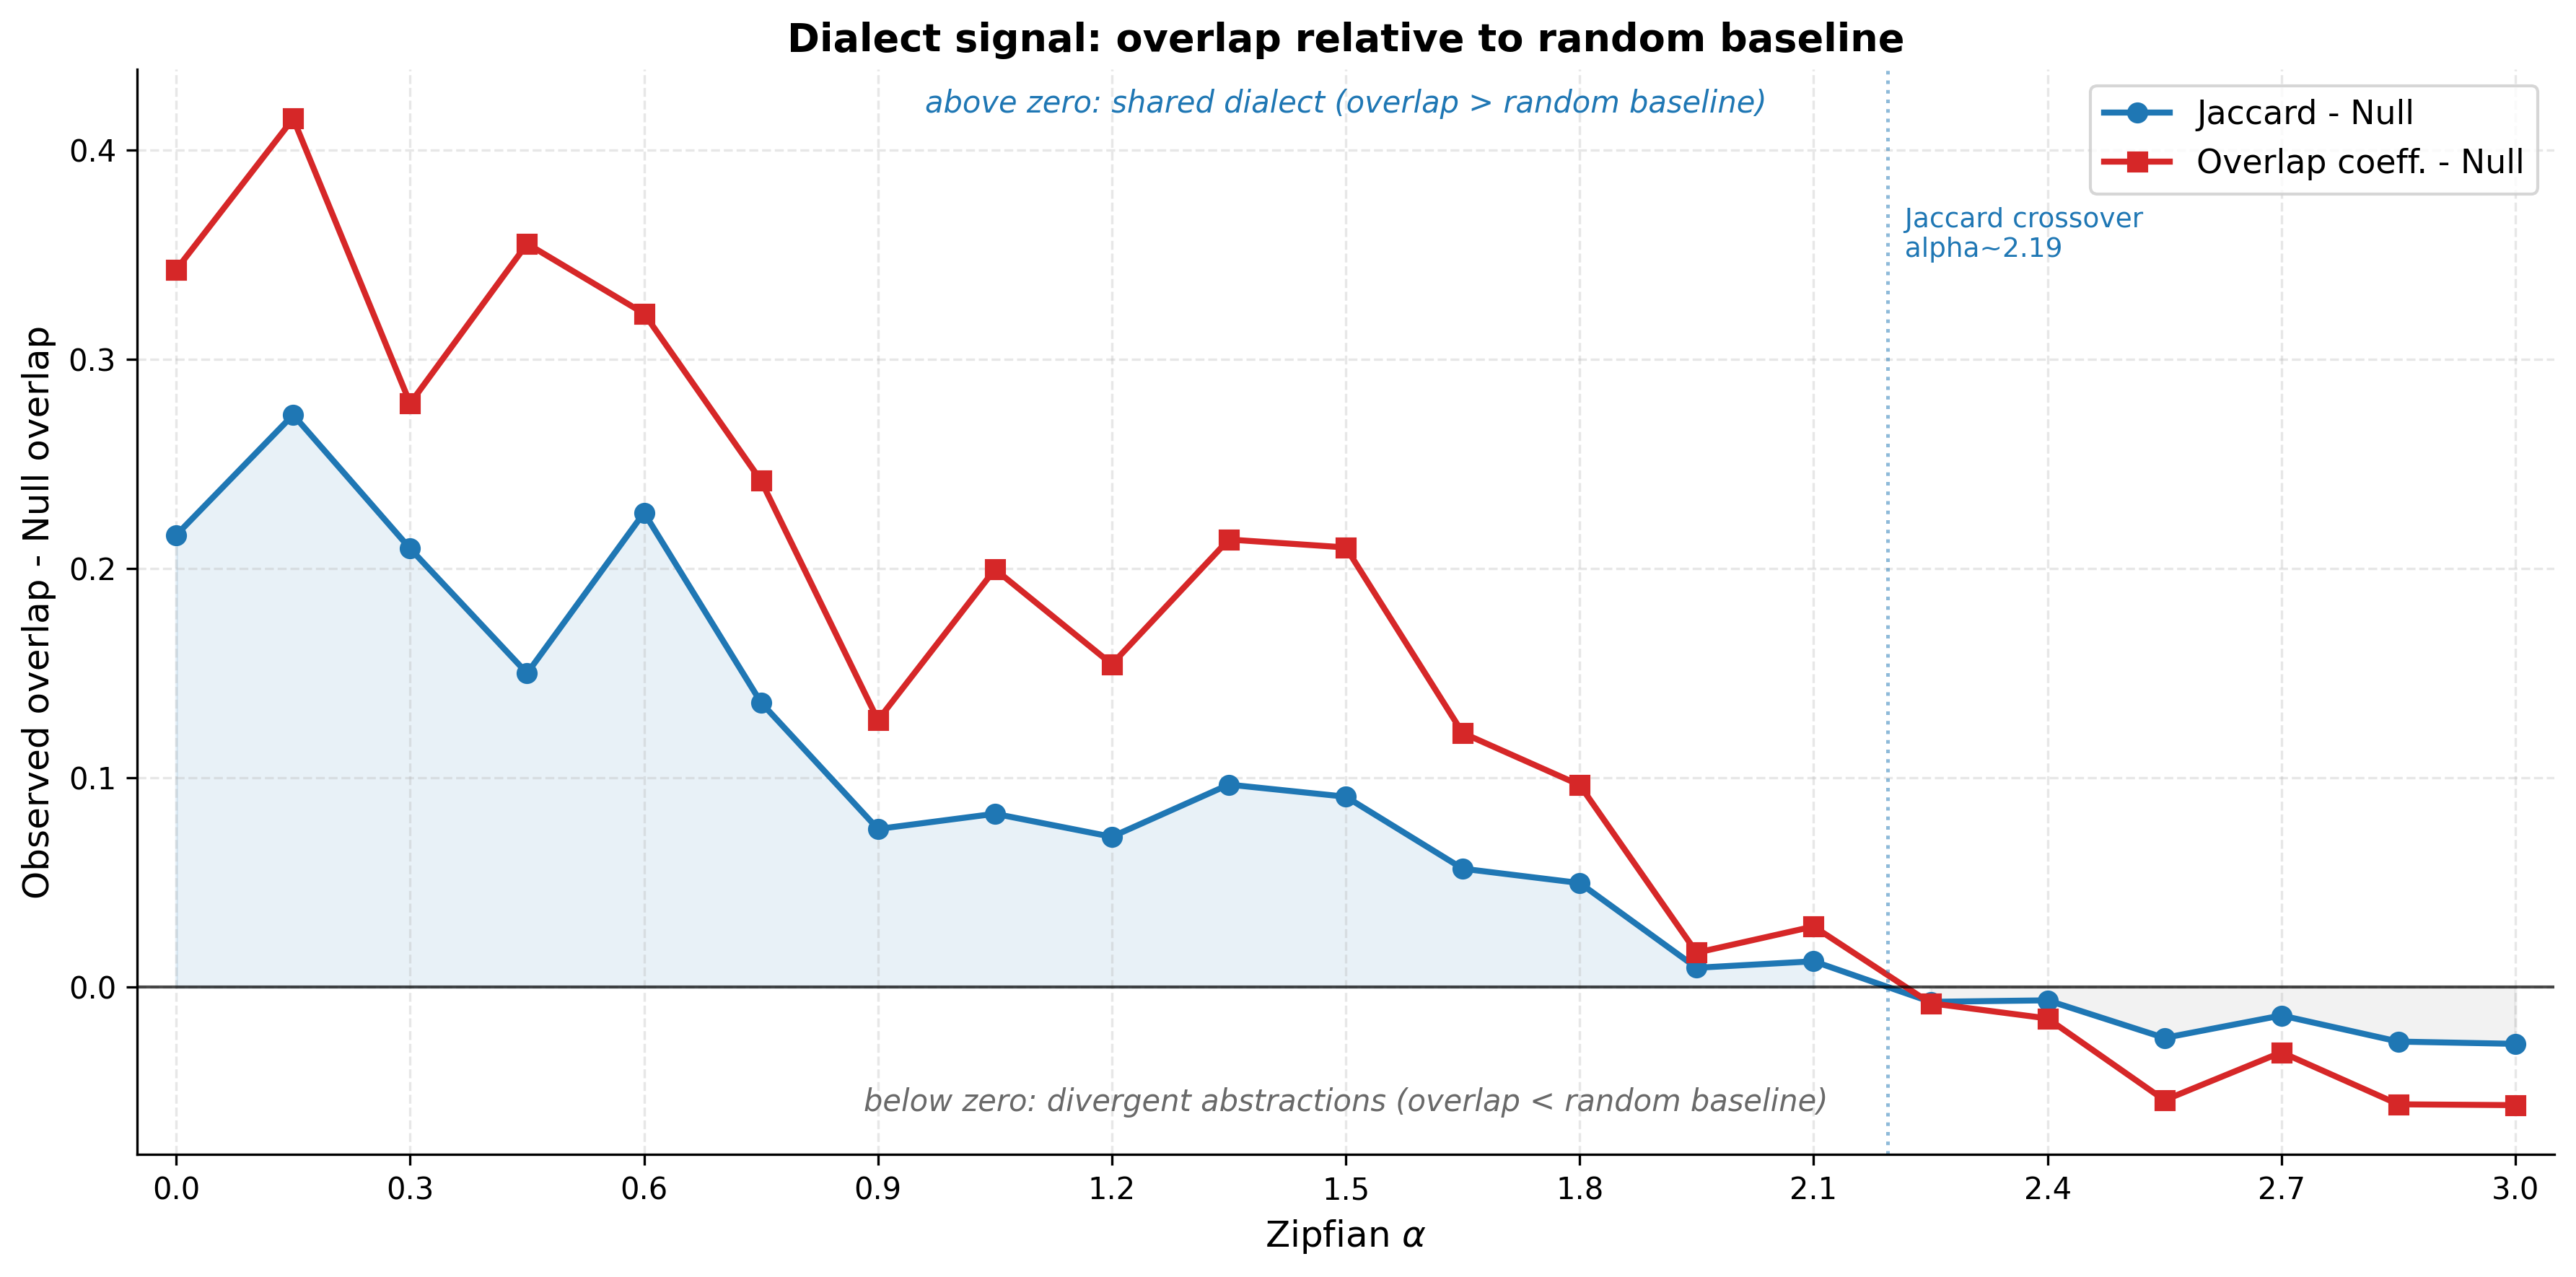
\includegraphics[width=0.88\textwidth]{images/overlap_minus_null.png}%
    }{%
        \missingfigure{images/overlap_minus_null.png}%
    }
    \caption{Dialect signal across the $\alpha$ range, defined as observed overlap minus null overlap. The crossover near $\alpha \approx 2.19$ marks the transition from above-chance convergence to below-chance divergence.}
    \label{fig:rq2-dialect-signal}
\end{figure}

This pattern admits a clear interpretation. In the low and moderate concentration regime, seeds genuinely converge on a common set of abstractions, and the library overlap exceeds what random sampling of the pool would produce. This is the dialect formation signature: shared structural pressure makes some abstractions universally attractive, regardless of which specific pairs happen to sit at the top of the ranking. In the high concentration regime, by contrast, the few abstractions each seed adopts are tightly tied to that seed's own top-ranked pairs. Because different seeds make different pairs frequent, their abstractions become idiosyncratic, and their libraries diverge from each other more than chance would predict. In short: low concentration produces shared vocabularies, high concentration produces private ones. Where you fall on this spectrum is determined entirely by $\alpha$.

\section{Pairwise Structure Across Seeds}
\label{sec:rq2-heatmaps}

The aggregate analysis of Section~\ref{sec:rq2-results} reports the mean and standard deviation of overlap across the 190 pairs. To see whether this average hides heterogeneity at the level of individual pairs, we compute the full pairwise overlap matrix at four representative $\alpha$ values, 0.00, 0.60, 1.80, and 3.00, and display them as heatmaps in Figure~\ref{fig:rq2-heatmaps}.

\begin{figure}[p]
    \centering
    \IfFileExists{images/heatmap_alpha_0.00.png}{%
        \begin{minipage}{0.48\textwidth}\centering
        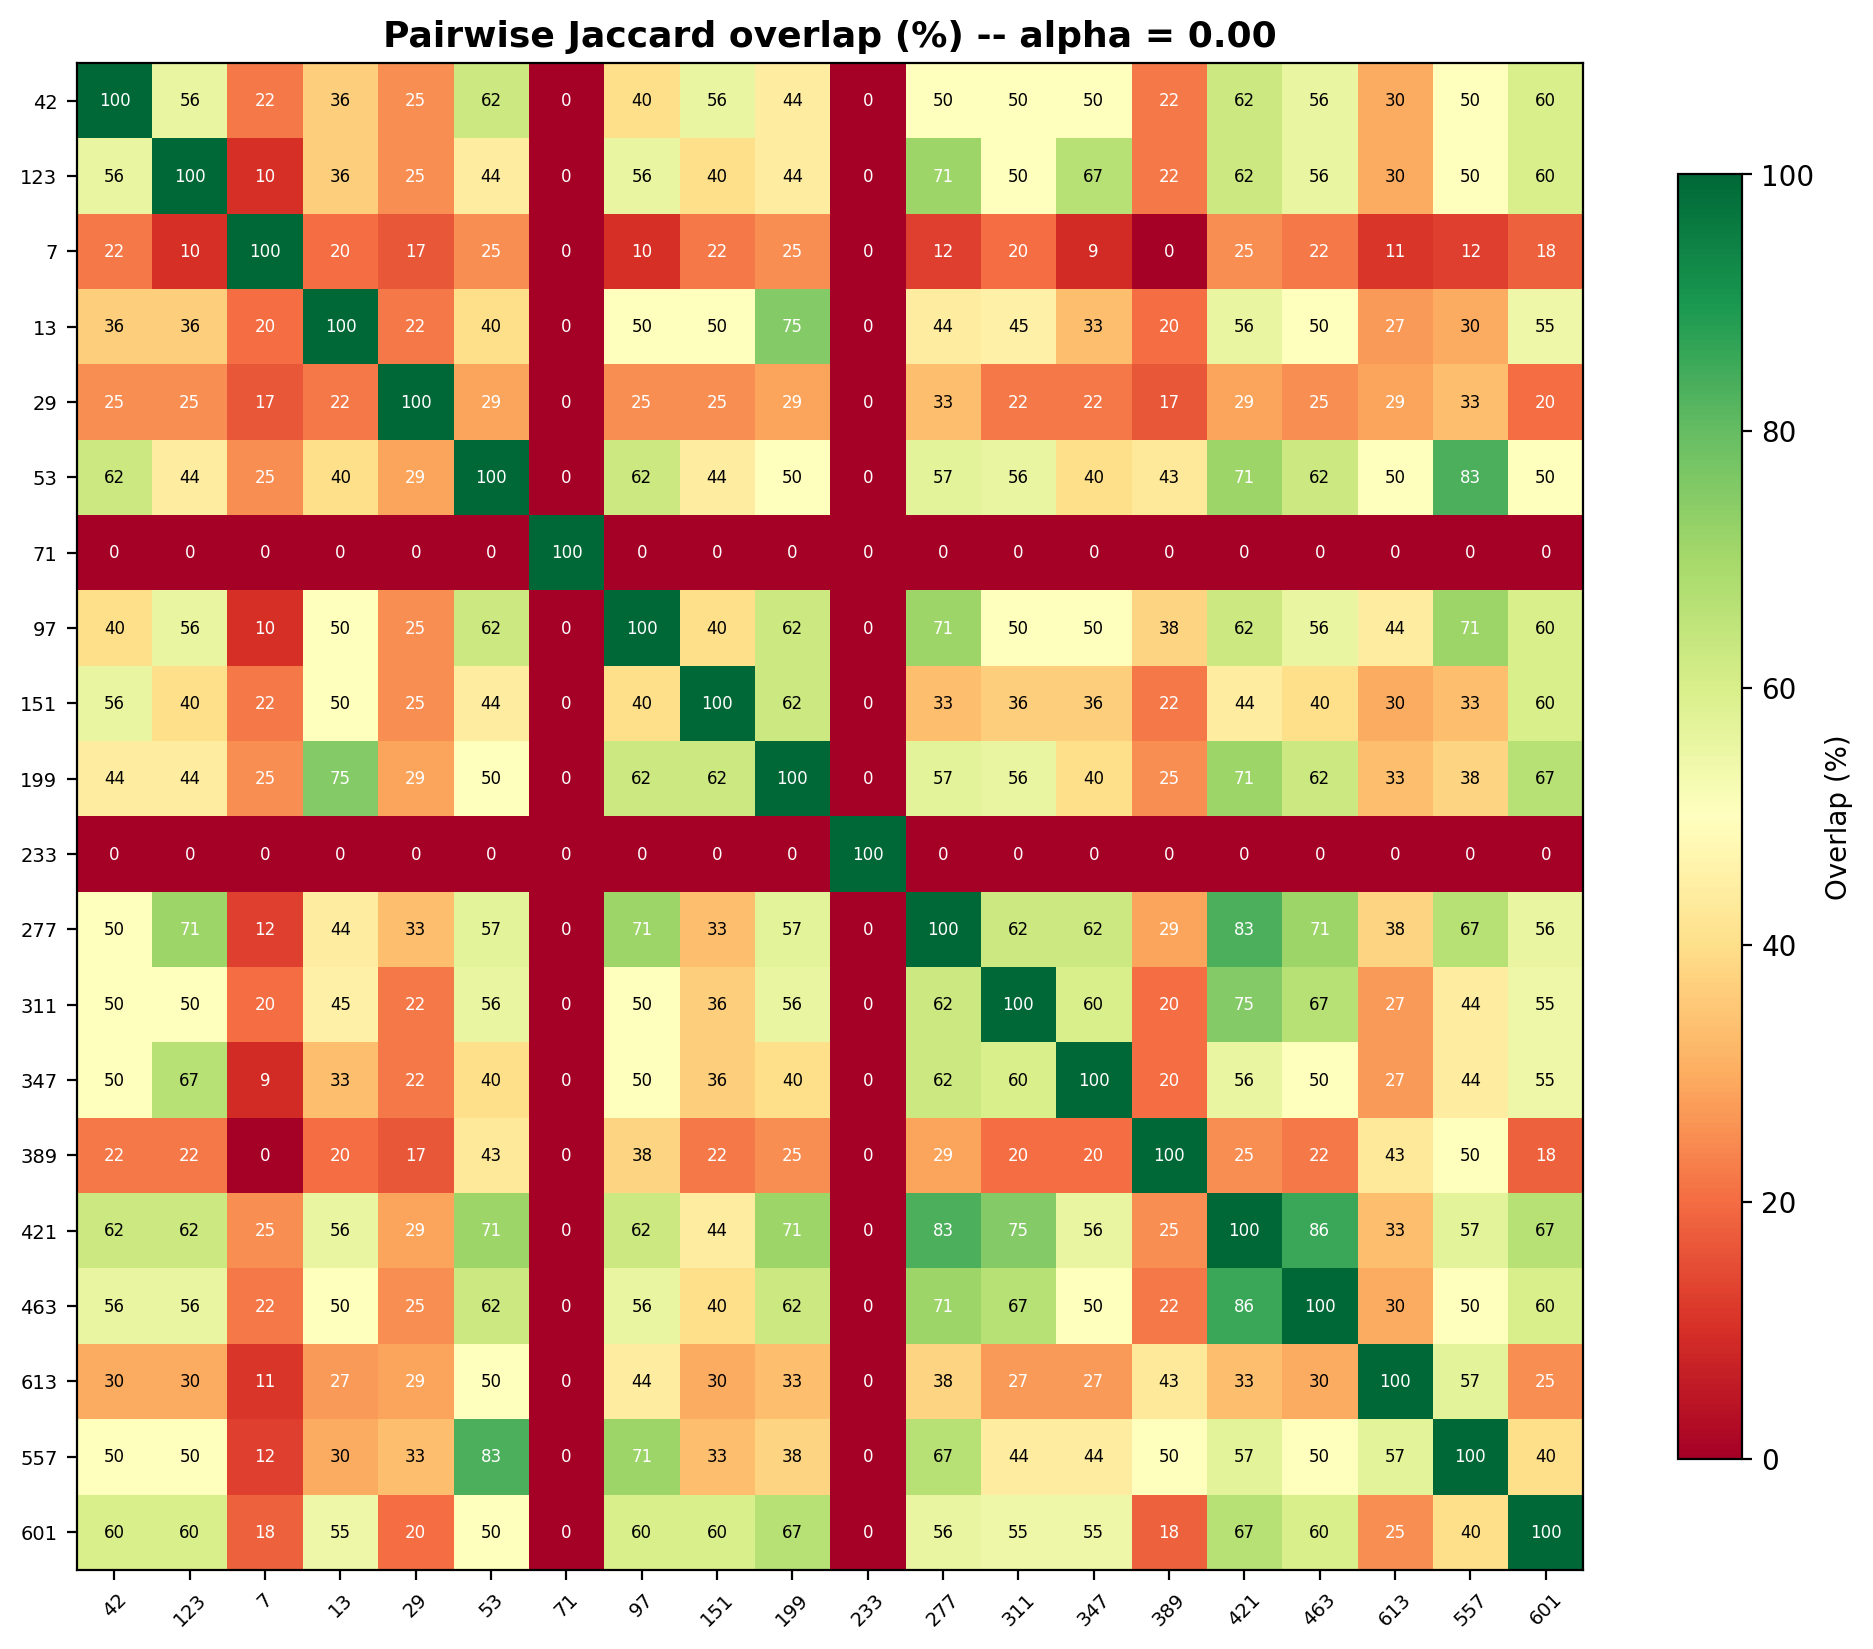
\includegraphics[width=\textwidth]{images/heatmap_alpha_0.00.png}
        \end{minipage}\hfill
        \begin{minipage}{0.48\textwidth}\centering
        \IfFileExists{images/heatmap_alpha_0.60.png}{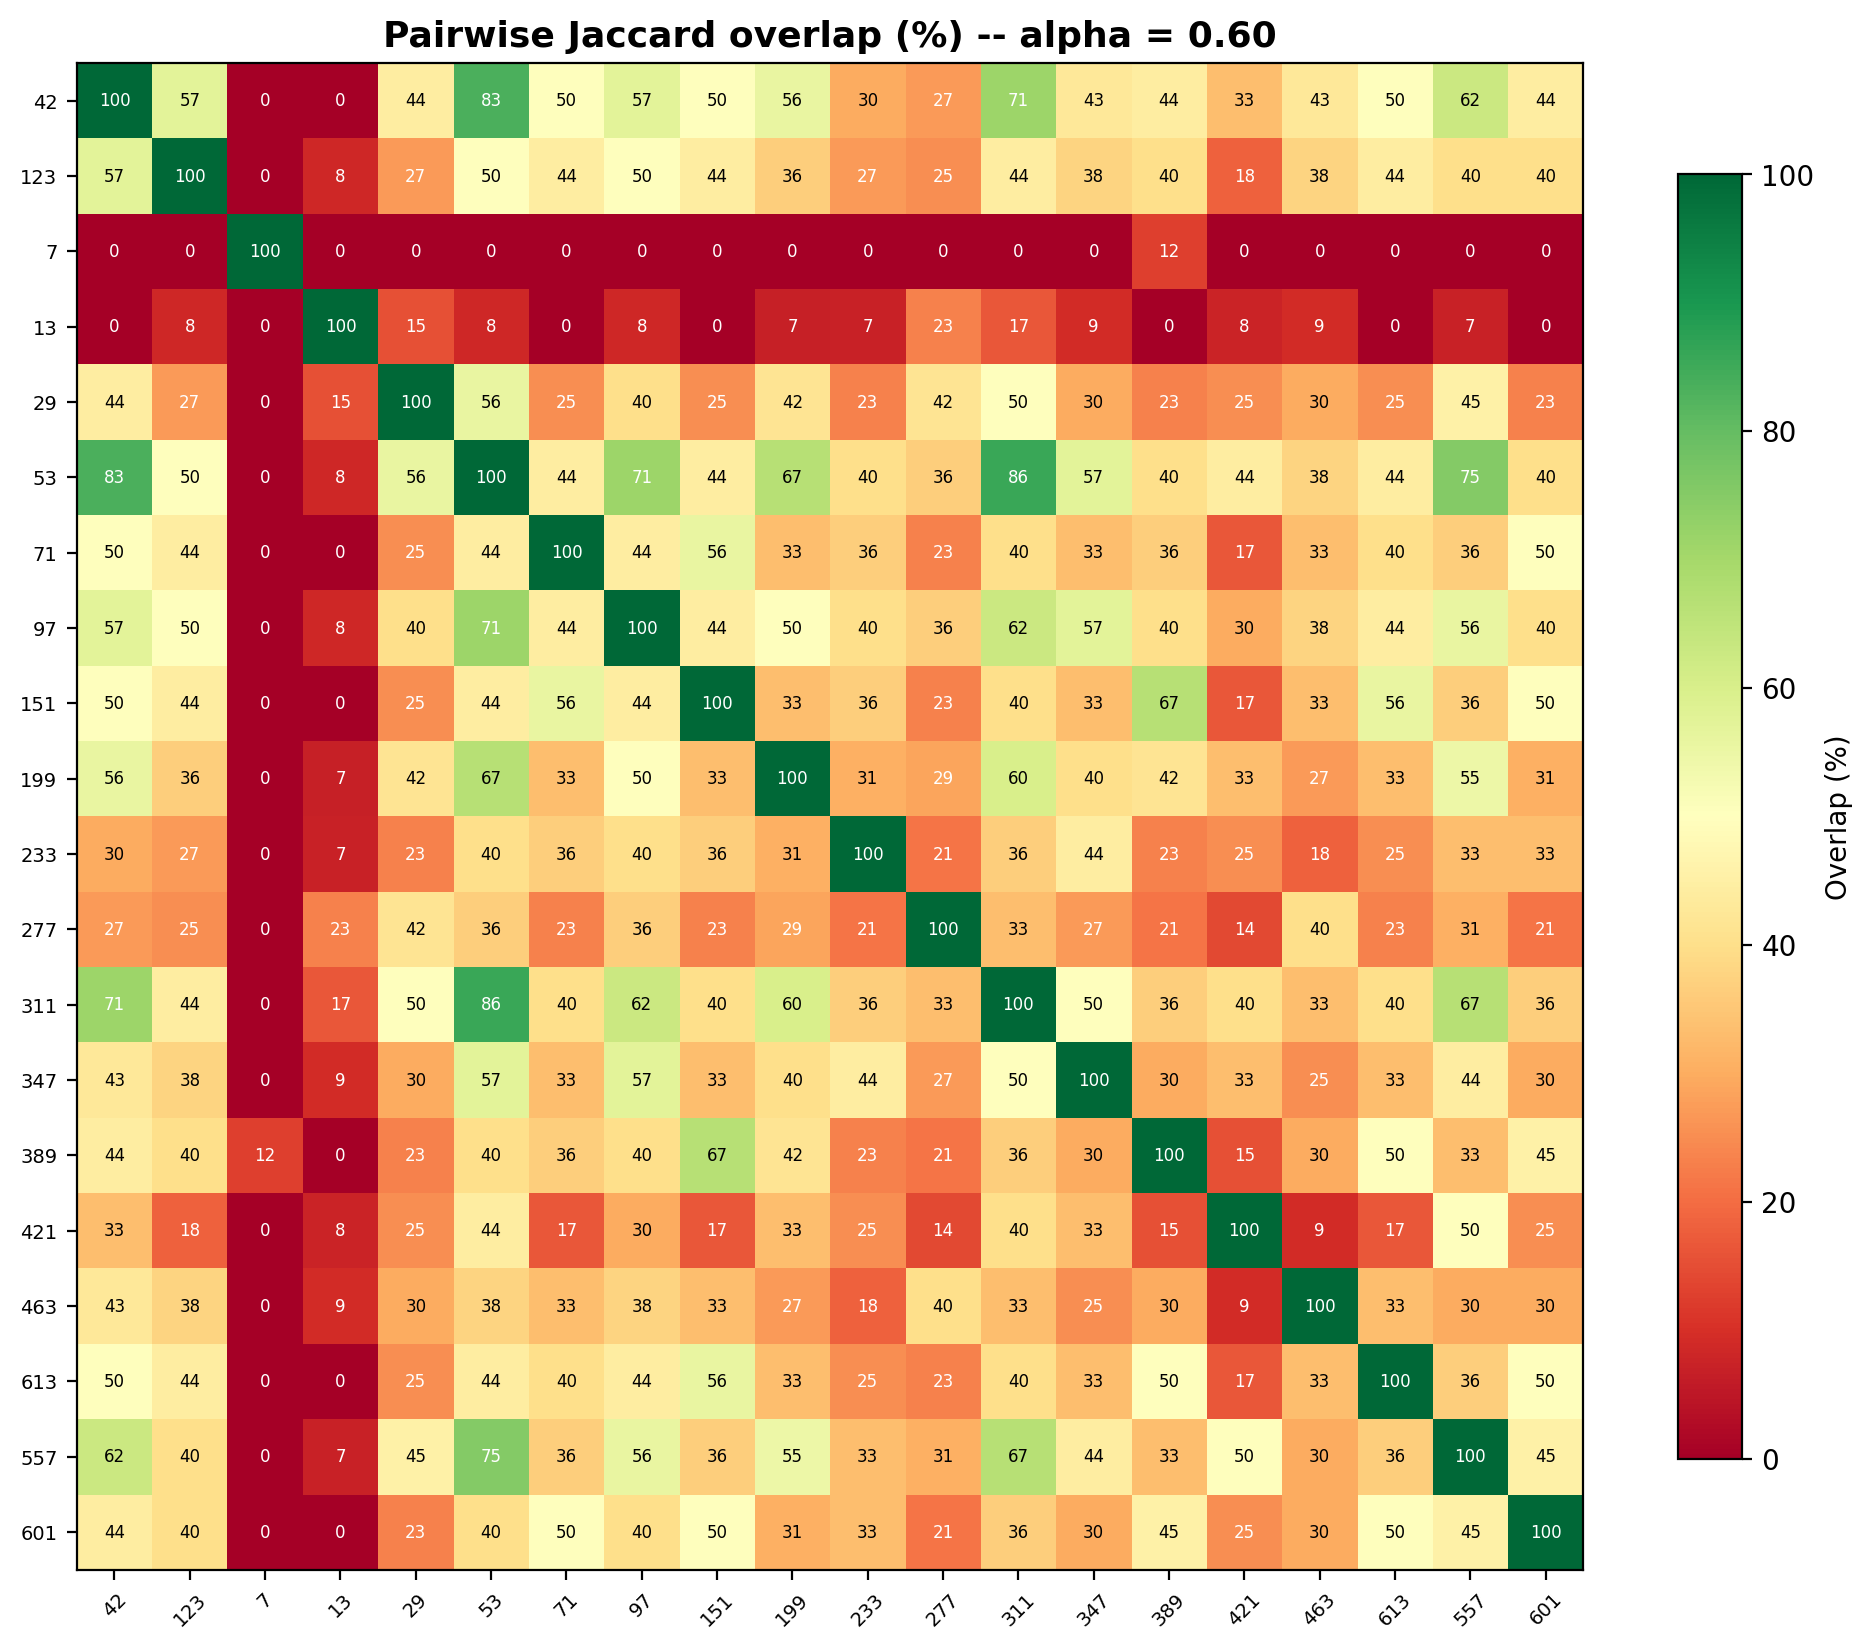
\includegraphics[width=\textwidth]{images/heatmap_alpha_0.60.png}}{\missingfigure{images/heatmap_alpha_0.60.png}}
        \end{minipage}

        \vspace{0.8em}

        \begin{minipage}{0.48\textwidth}\centering
        \IfFileExists{images/heatmap_alpha_1.80.png}{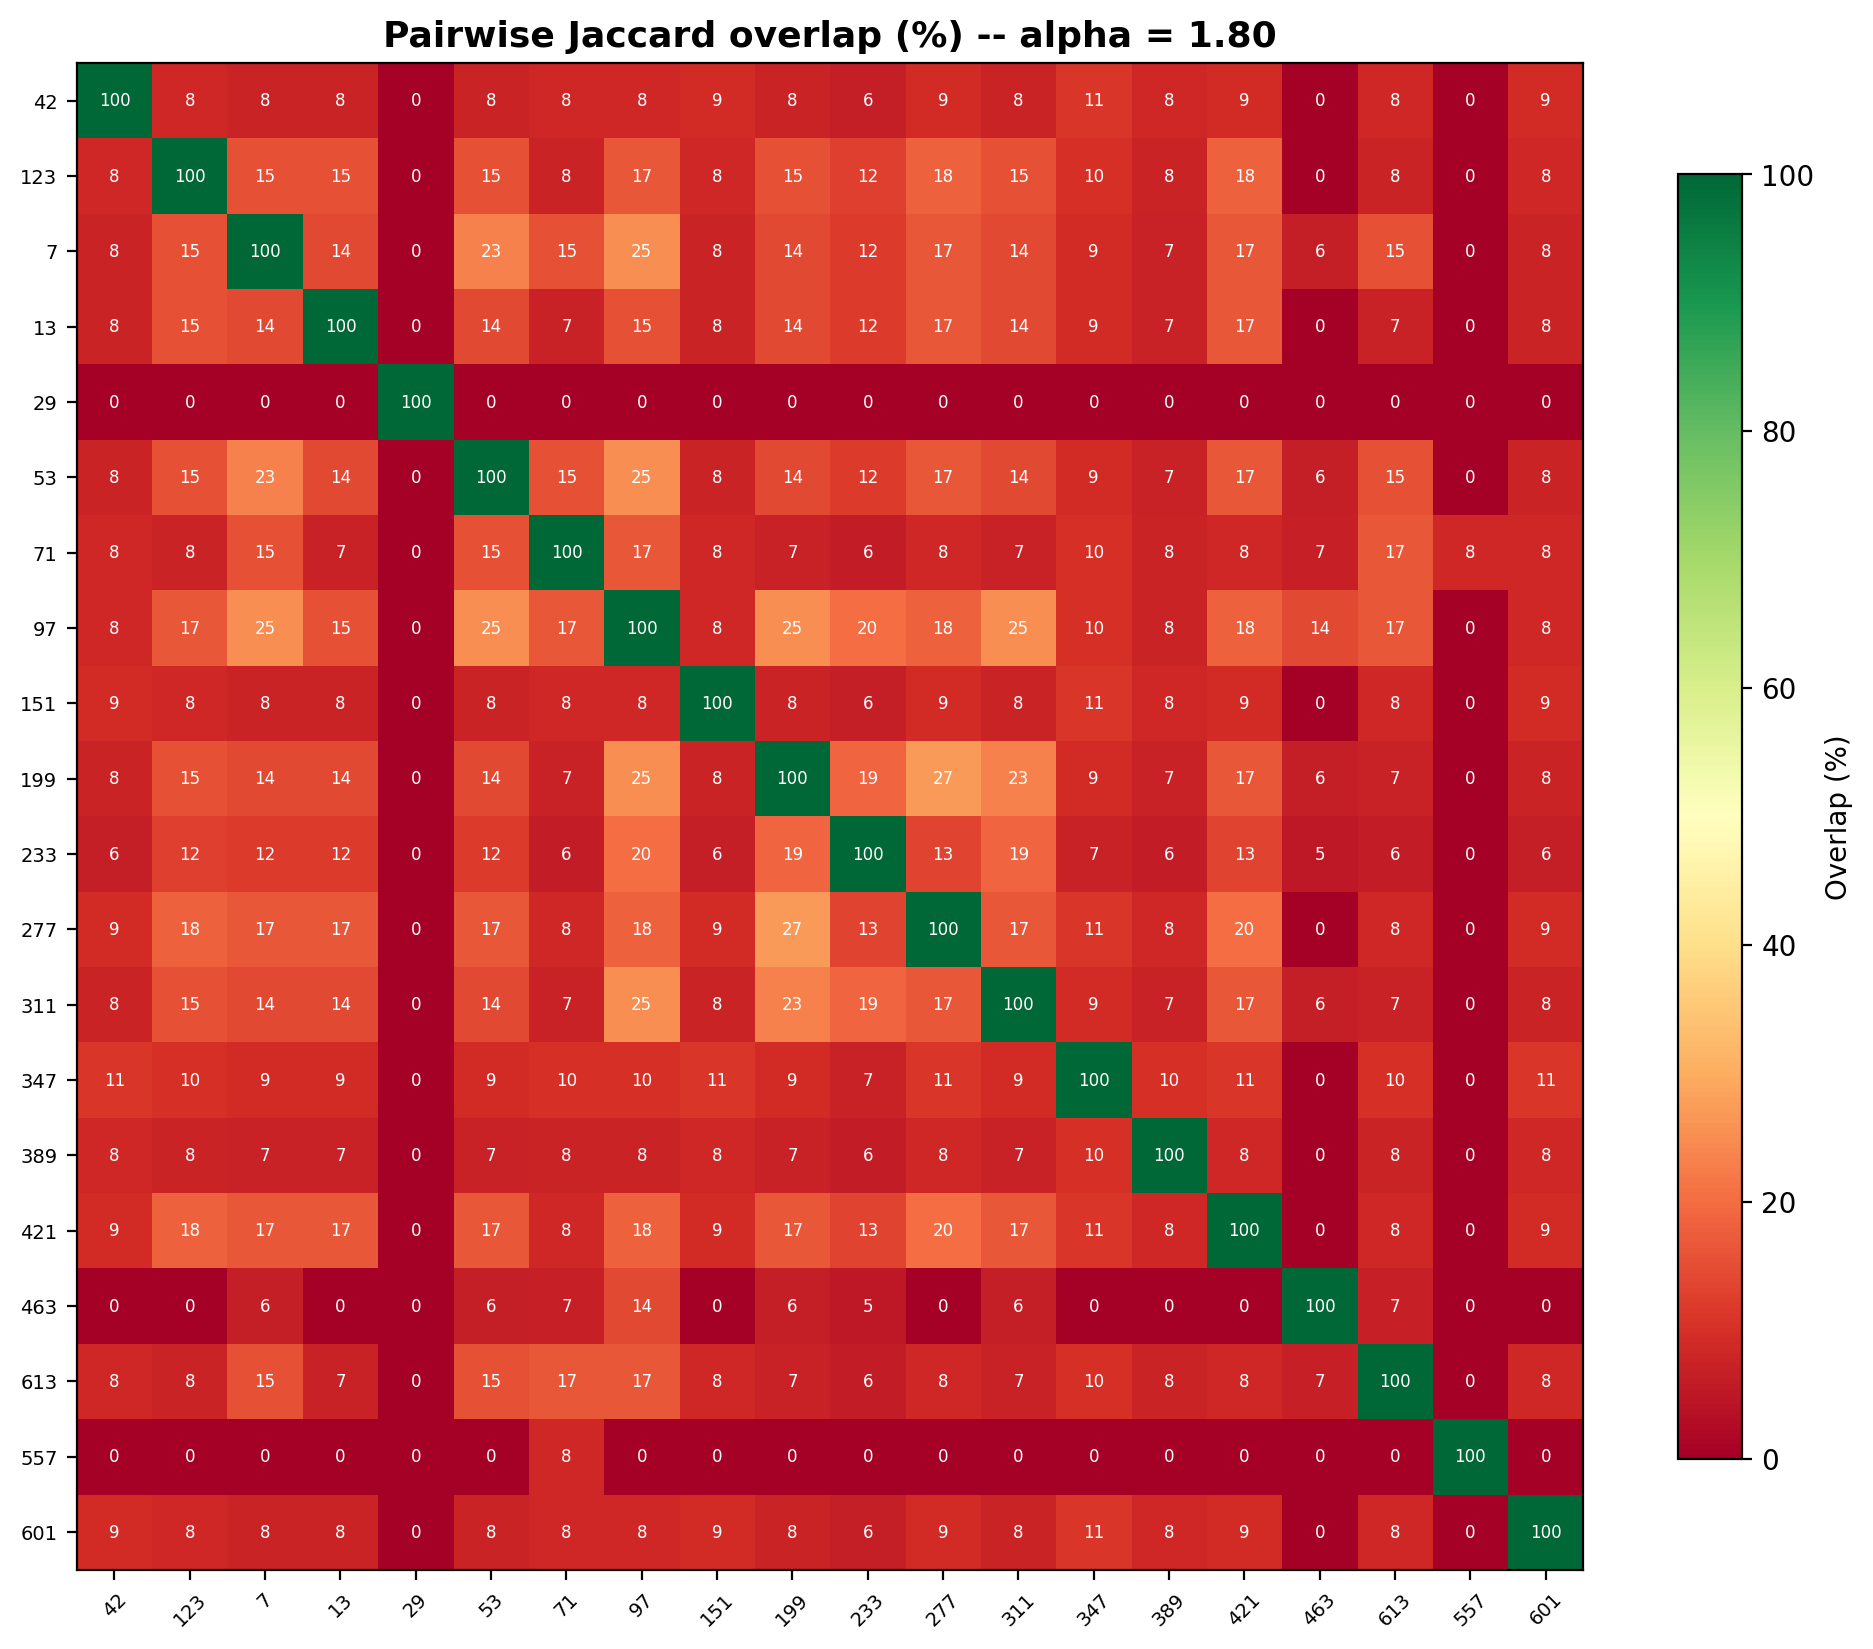
\includegraphics[width=\textwidth]{images/heatmap_alpha_1.80.png}}{\missingfigure{images/heatmap_alpha_1.80.png}}
        \end{minipage}\hfill
        \begin{minipage}{0.48\textwidth}\centering
        \IfFileExists{images/heatmap_alpha_3.00.png}{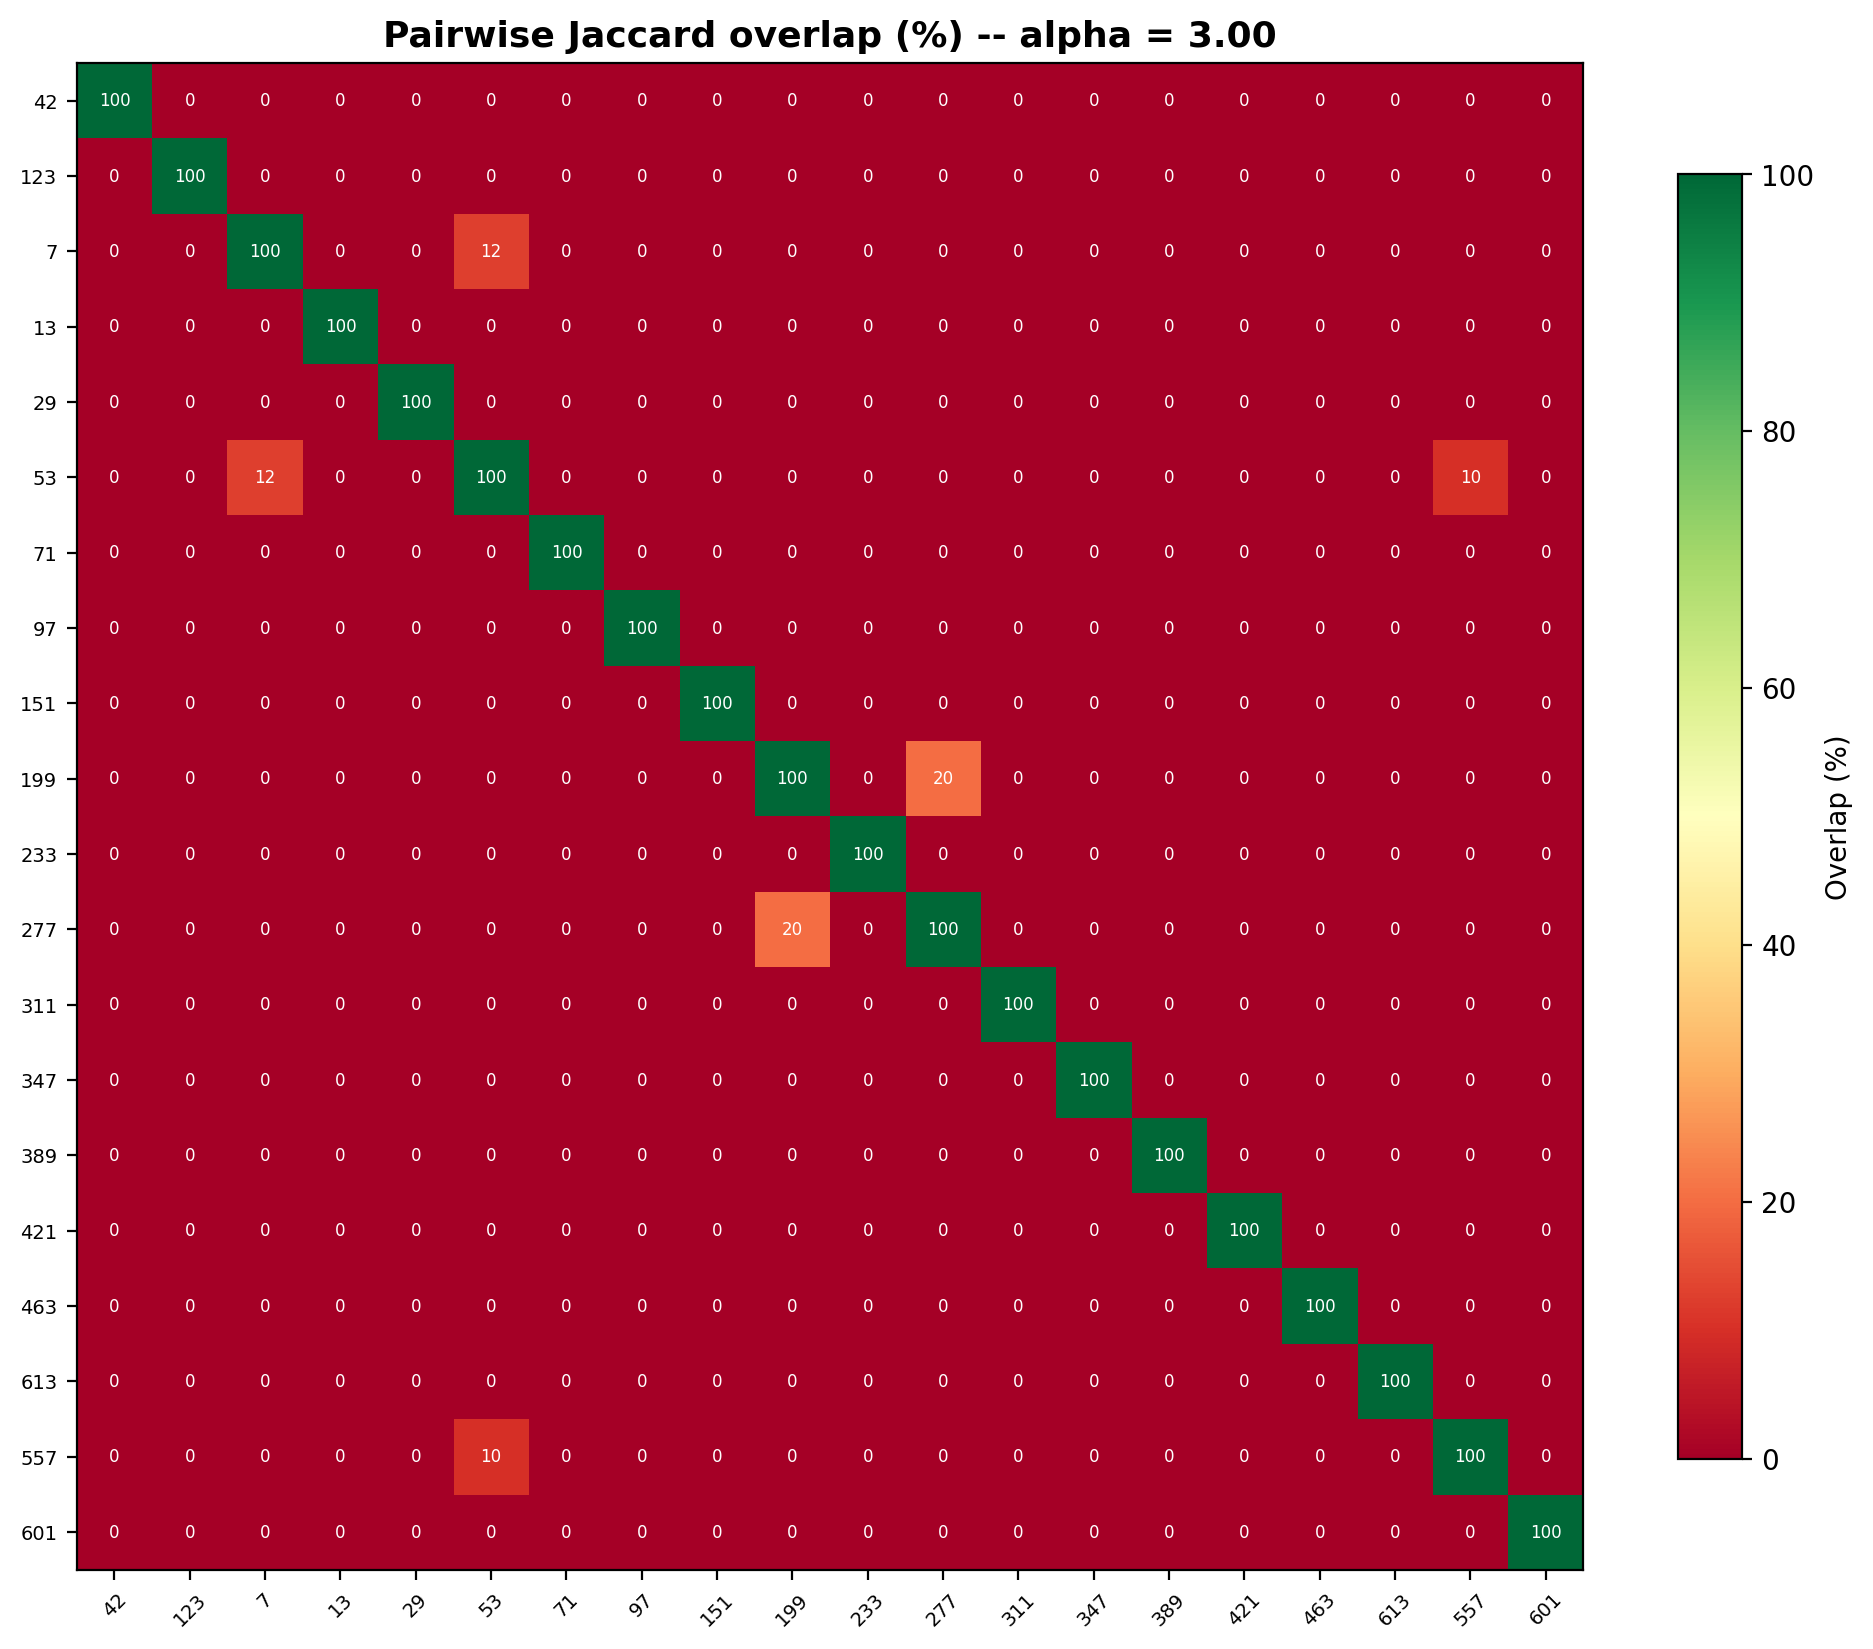
\includegraphics[width=\textwidth]{images/heatmap_alpha_3.00.png}}{\missingfigure{images/heatmap_alpha_3.00.png}}
        \end{minipage}
    }{%
        \begin{minipage}{0.48\textwidth}\centering
        \missingfigure{images/heatmap_alpha_0.00.png}
        \end{minipage}\hfill
        \begin{minipage}{0.48\textwidth}\centering
        \missingfigure{images/heatmap_alpha_0.60.png}
        \end{minipage}

        \vspace{0.8em}

        \begin{minipage}{0.48\textwidth}\centering
        \missingfigure{images/heatmap_alpha_1.80.png}
        \end{minipage}\hfill
        \begin{minipage}{0.48\textwidth}\centering
        \missingfigure{images/heatmap_alpha_3.00.png}
        \end{minipage}
    }
    \caption{Pairwise Jaccard overlap heatmaps at four representative concentration levels: $\alpha = 0.00$, $0.60$, $1.80$, and $3.00$. Together they show the transition from a broadly shared library to strongly seed-specific dialects.}
    \label{fig:rq2-heatmaps}
\end{figure}

At $\alpha = 0.00$, most cells sit in the 0.20 to 0.60 Jaccard range, and the heatmap has the visual appearance of a broadly convergent population. Two seeds, 71 and 233, stand out as having essentially zero overlap with all other seeds. These are not random outliers with low overlap against one or two other seeds; they are systematically isolated. Inspection of their libraries shows that both adopted abstractions that almost no other seed picked up at $\alpha = 0.00$. The most likely mechanism is the bandit's exploration branch: at low $\alpha$, where many candidates have similar MDL scores, $\varepsilon$-greedy exploration occasionally locks onto unconventional choices that the rest of the population does not follow. Because the candidate pool at low $\alpha$ is large, this cost is invisible within each run, but it shows up sharply when the libraries are compared across populations. We keep these seeds in all aggregate statistics rather than excluding them, because their behaviour reflects a real feature of the bandit-based adoption mechanism.

At $\alpha = 0.60$ the heatmap shows a similar global structure but with weaker alignment. Local clusters of mutually agreeing seeds remain visible, and some pairs reach Jaccard values above 0.70, but other seeds start dropping toward zero overlap with most of the population. The transition from a coherent global library at $\alpha = 0.00$ to a more fragmented one at $\alpha = 0.60$ is consistent with the gradual decrease in mean overlap of Section~\ref{sec:rq2-results}.

At $\alpha = 1.80$ the heatmap is dominated by low values, mostly between 0.05 and 0.25. The few exceptions are pairs of two or three seeds that happen to share several abstractions. Three seeds, 29, 463, and 557, show essentially zero overlap with all others. The dialect signal identified in Section~\ref{sec:rq2-results} for this $\alpha$ is therefore not produced by uniform agreement across all pairs, but by partial agreement among many pairs combined with a handful of isolated seeds.

At $\alpha = 3.00$ the heatmap is almost entirely empty except for the diagonal. Most pairs share zero abstractions, with only a few cells showing values in the 0.10 to 0.20 range. These rare non-zero cells correspond to pairs of seeds that happened to share one or two abstractions among the small libraries that survived in this regime. The matrix as a whole confirms that at very high concentration, each seed develops an essentially private library that other seeds do not reproduce.

The progression across the four heatmaps mirrors the dialect signal trajectory: a coherent shared dialect at $\alpha = 0.00$, gradual fragmentation through the moderate range, and complete divergence at $\alpha = 3.00$.

\section{Qualitative Analysis at $\alpha = 1.50$}
\label{sec:rq2-qualitative}

The quantitative evidence of Sections~\ref{sec:rq2-results} and~\ref{sec:rq2-heatmaps} establishes that libraries diverge with $\alpha$. The qualitative question that follows is why. Do the abstractions adopted by each seed track the structural properties of the pairs that seed makes frequent, in a way we can see directly by inspecting the libraries? If yes, the divergence is not a stochastic artefact of bandit exploration or neural initialisation, it is a reflection of the input distribution operating through the MDL score.

We look at $\alpha = 1.50$ for this analysis, because it sits in the moderate-concentration regime where the dialect signal is still positive but seed-specific identity already matters. Under seed 42, the most frequent shape pair is \texttt{lower\_a upper\_j} with frequency 377, followed by \texttt{upper\_t upper\_c} with frequency 134 and \texttt{upper\_l lower\_u} with frequency 73. Under seed 123, the top-ranked pairs are entirely different: \texttt{upper\_d upper\_o} with frequency 377, \texttt{lower\_v lower\_x} with frequency 134, and \texttt{upper\_n upper\_h} with frequency 73. The identity of the dominant pairs is fixed by the seed-based permutation, while the frequency profile is identical between the two.

Inspection of the adopted libraries at $\alpha = 1.50$ shows a clear correspondence between the dominant pairs and the abstractions the bandit adopts during the early proposal steps. Under seed 42, the first abstractions to be adopted include subsequences that appear inside the construction of the top-ranked pairs. For example, the abstraction \texttt{[[1,0],[0,1]]} is a subsequence of the action sequence used to construct \texttt{lower\_a upper\_j}, seed 42's rank-1 pair. Under seed 123, the analogous early abstraction is \texttt{[[1,0],[1,0]]}, the classical tower shape, which appears in all five top-ranked pairs of that seed. This pattern holds for the first four to five adoption decisions, which consistently correspond to sub-structures of the seed-specific top pairs.

Beyond the fifth adoption the picture becomes more complex. By that stage the candidate pool already contains composite tokens referring to abstractions that were adopted in earlier proposal steps, so later abstractions are no longer simple primitive sequences but rather sequences over a mixed vocabulary of primitives and compound tokens. At this point the surface form of an abstraction does not directly match a top-ranked pair, but its internal composition still reflects the structural patterns that the corresponding seed made frequent. The two seeds continue to diverge from each other in a way that tracks the underlying need distribution, even when the divergence is no longer easily readable at the level of primitive subsequences.

This qualitative reading supports a stronger interpretation of the quantitative results. The decreasing overlap between seeds is not a stochastic artefact. It reflects the fact that different seeds make different shape pairs frequent, and these different pairs make different subsequences attractive under the MDL criterion. The libraries different populations produce are procedural dialects in a substantive sense: each is shaped by the specific need distribution of the population that produced it.

\section{Library Change Within the Same Seed Across $\alpha$}
\label{sec:rq2-intraseed}

The analysis so far compares different seeds at a fixed $\alpha$. A complementary question is how a single seed's library changes as $\alpha$ itself varies. The two analyses probe related but distinct sources of variability. The cross-seed analysis fixes $\alpha$ and varies the ranking, isolating the effect of which pairs are made frequent. The within-seed analysis fixes the ranking and varies $\alpha$, isolating the effect of how concentrated the frequency profile is.

We compute, for seed 42, the Jaccard index between the library adopted at $\alpha = 0.00$, used as reference, and the library adopted at each other $\alpha$ value. Figure~\ref{fig:rq2-intraseed-overlap} reports the result.

\begin{figure}[htbp]
    \centering
    \IfFileExists{images/overlap_vs_alpha_intraseed.png}{%
        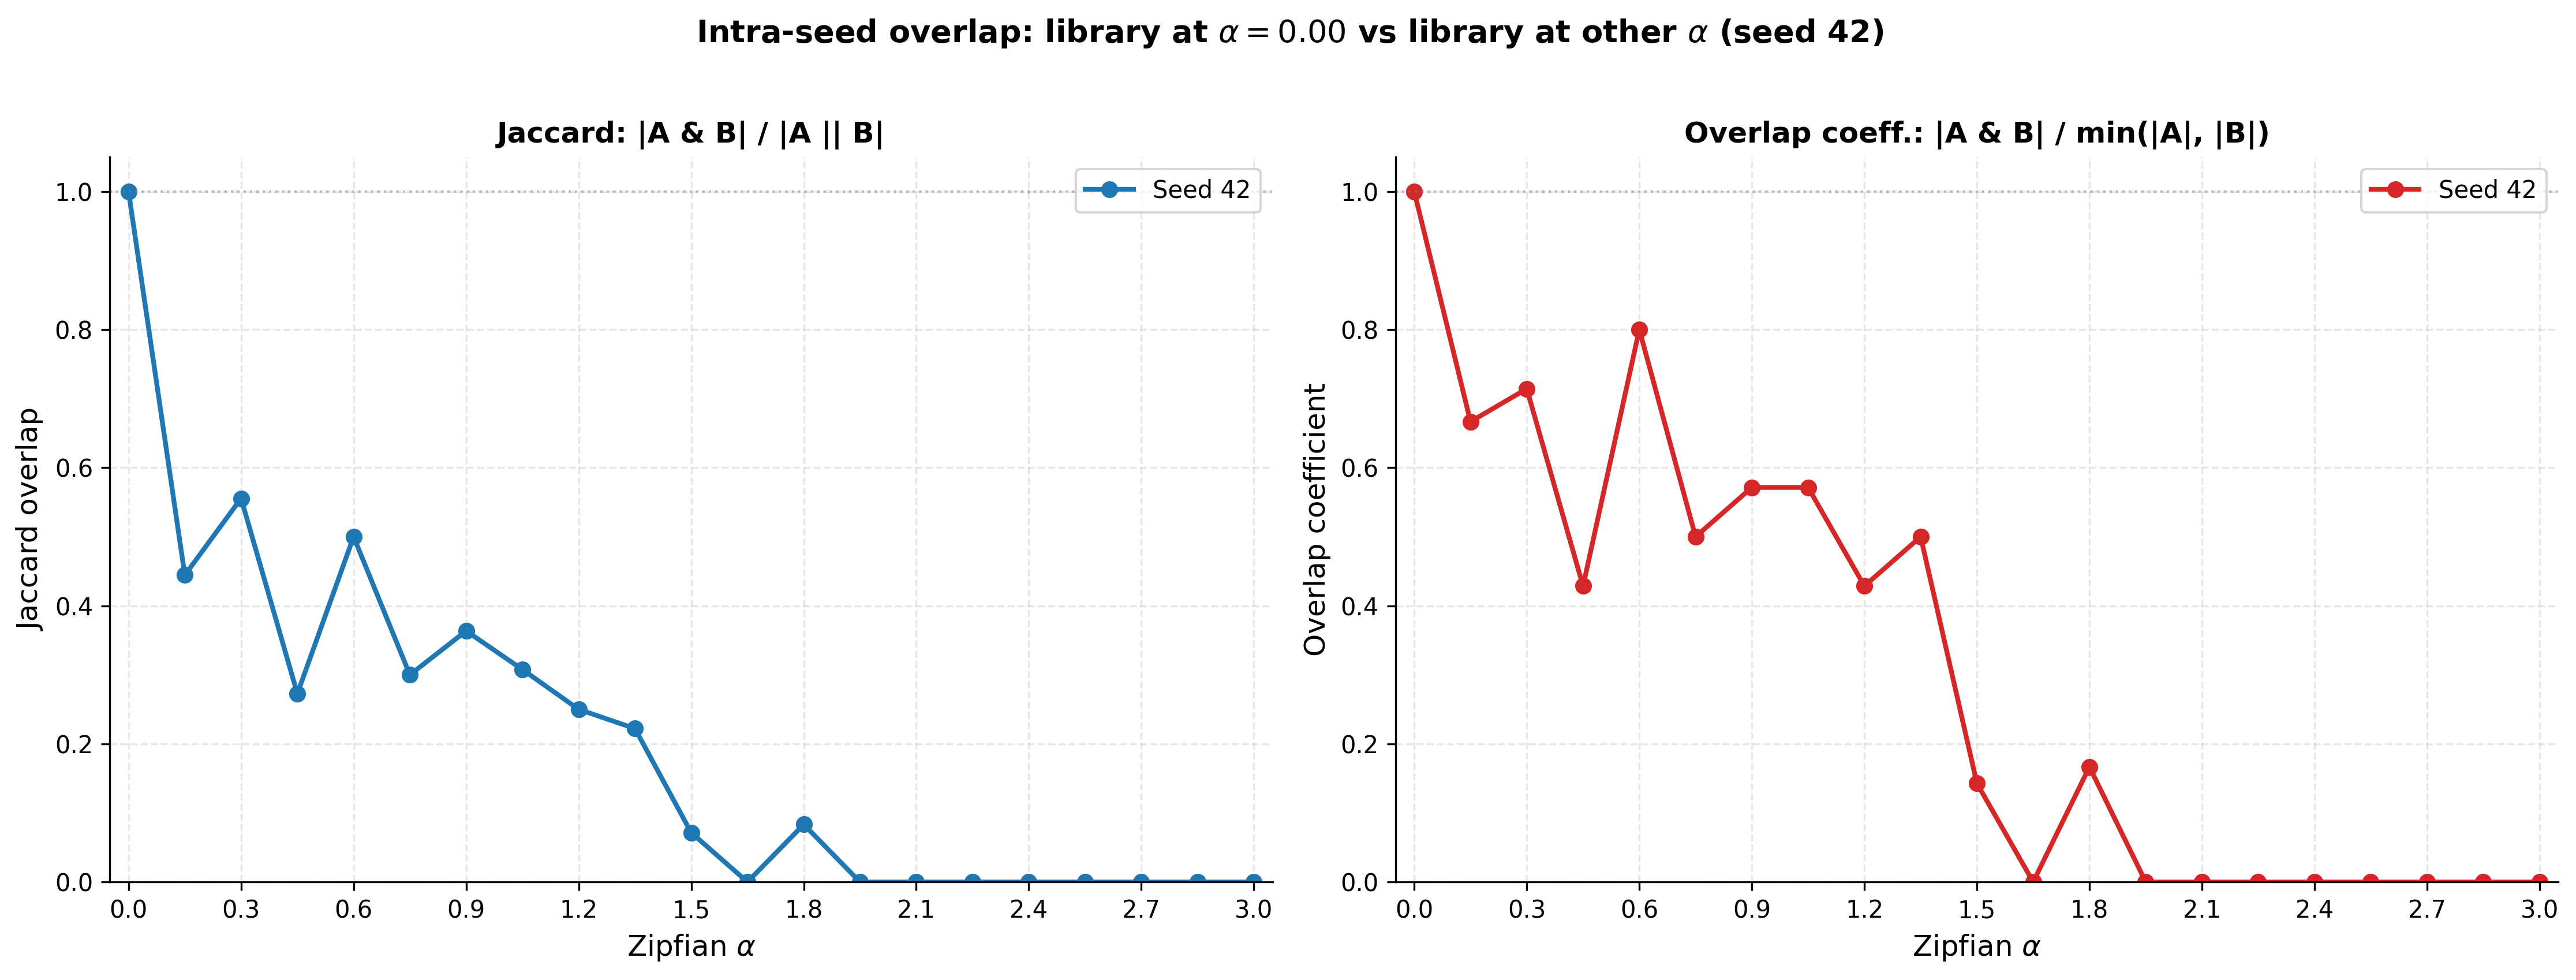
\includegraphics[width=0.95\textwidth]{images/overlap_vs_alpha_intraseed.png}%
    }{%
        \missingfigure{images/overlap_vs_alpha_intraseed.png}%
    }
    \caption{Library overlap as a function of $\alpha$ for seed 42, computed with respect to the reference library at $\alpha = 0.00$.}
    \label{fig:rq2-intraseed-overlap}
\end{figure}

The Jaccard starts at 1.0 by construction at $\alpha = 0.00$ and drops sharply to about 0.45 already at $\alpha = 0.15$. Through the moderate range, the Jaccard oscillates between 0.30 and 0.55 without a clear monotone trend, then falls more steeply above $\alpha = 1.50$ and reaches zero by $\alpha = 1.65$. It remains at or near zero for all higher concentrations. The overlap coefficient follows a similar trajectory but with systematically higher values, reflecting the fact that it does not penalise size differences.

The point-to-point oscillation in the moderate range is partly stochastic: each point comes from a single PACE run, not from an average across independent replicates. The single-run version reported here is sufficient to establish the qualitative pattern, but the individual oscillations should be read with corresponding caution.

One qualitative observation is worth highlighting. The abstraction \texttt{[[1,0],[0,1]]}, which represents the minimal composition of two orthogonal primitive drawings, appears in the library of seed 42 at $\alpha = 0.00$, $\alpha = 1.50$, and $\alpha = 1.80$. No other abstraction is shared across all three of these regimes. This pattern is the simplest non-trivial composition PACE can adopt, and its persistence across qualitatively different distributional regimes suggests that it functions as a canonical chunk: a recurring procedural shape that PACE finds useful regardless of which specific pairs become dominant. The fact that all other abstractions are regime-specific reinforces the broader picture: libraries are tightly tied to the structural composition of the pairs that each concentration profile makes frequent.

The within-seed analysis therefore confirms the cross-seed picture from a different angle. Two seeds at the same $\alpha$ share around a third of their libraries at low concentration and essentially nothing at high concentration. The same seed across different $\alpha$ values follows a comparable trajectory: its library at $\alpha = 0.15$ already overlaps with its $\alpha = 0.00$ reference by only 0.45 in Jaccard terms, and the overlap collapses to zero for $\alpha \geq 1.65$. Both axes of variation produce comparable degrees of library divergence, which suggests that the distributional context, in both its ranking and its concentration components, exerts a strong and pervasive effect on the resulting library.

\section{Discussion}
\label{sec:rq2-summary}

The results of this chapter give a coherent account of dialect formation under Zipfian input. Library overlap decreases smoothly as $\alpha$ increases, unlike the non-monotone adoption-count pattern of RQ1. Both Jaccard and overlap coefficient follow this trend, with correlations close to $-0.98$ and highly significant $p$-values. The null model adds the key transition: up to about $\alpha = 2.19$, seeds share more abstractions than chance would predict, suggesting a common structural backbone; above that point, overlap falls below the null and libraries become tied to seed-specific top pairs. The qualitative analysis at $\alpha = 1.50$ explains why. Early abstractions appear as sub-structures of each seed's top-ranked pairs, and later abstractions carry the same seed-specific structure through compound tokens. The within-seed comparison in Section~\ref{sec:rq2-intraseed} reinforces the same conclusion: both ranking and concentration leave direct traces in the library the bandit builds.

Two notes of caution. The first concerns interpretation at high $\alpha$. The negative dialect signal for $\alpha$ > 2.19 does not mean that populations are actively pushing away from each other. It reflects the fact that libraries at high $\alpha$ are small, as Chapter~\ref{ch:experimental} reported a mean of about 3.6 adopted abstractions at $\alpha = 3.00$, and small libraries tied to a handful of frequent pairs are almost mechanically going to look more idiosyncratic than random subsets of a shared pool. The observed pattern is consistent with dialect formation at both ends of the range, but the high-$\alpha$ dialects are more impoverished than the moderate-$\alpha$ ones.

These results also set up the communication question. If dialects are functional local communication systems, then interaction across populations should degrade as library divergence increases, with high $\alpha$ producing the most severe failures. Chapter~\ref{ch:rq3} uses this as the starting prediction, then complicates it: adaptation difficulty does not scale cleanly with pairwise distributional distance, and cross-$\alpha$ asymmetries are driven by the specificity of the speaker's library rather than by raw speaker-listener divergence. The dialect analysis here supplies the vocabulary for that result, even though the communication experiments resist the simplest divergence-to-failure story.